\chapter{Contenidos teóricos}

En los siguientes apartados se explican los contenidos claves de este proyecto, que son la computación cuántica\ \ref{sec:intro:cc}, la tecnología \textit{blockchain}\ \ref{sec:intro:blockchain} y el algoritmo \acrshort{uov}\ \ref{sec:intro:UOV}.

\section{Computación cuántica}\label{sec:intro:cc}

La evolución de la tecnología se ha basado principalmente en la reducción de los transistores para aumentar la velocidad, llegando a escalas de tan solo algunas decenas de nanómetros. Esto tiene un límite y es la eficiencia, puesto que al seguir disminuyendo el tamaño podrían dejar de funcionar correctamente. De ahí surge la necesidad de descubrir nuevas tecnologías, la computación cuántica \cite{computacion-cuantica-wiki}. Así, la computación cuántica constituye un nuevo paradigma de la informática basado en los principios de la teoría cuántica.\\

Las tecnologías cuánticas nacieron del estudio de algunos fenómenos físicos que aún no se entendían bien, entre los años 1900 y 1930, dando lugar a una nueva teoría en la física, la Mecánica Cuántica. La Mecánica Cuántica es la rama de la física que estudia del mundo microscópico, los sistemas atómicos y subatómicos y su interacción con la radiación electromagnética \cite{mecanica-cuantica}.

\subsection{Historia}

La computación cuántica tuvo sus inicios en los años 50 cuando algunos físicos, como Richard Feynman, fueron pioneros en mencionar posibilidad de utilizar efectos cuánticos para realizar cálculos computacionales \cite{computacion-cuantica-wiki}. En la charla de Richard Feynman titulada ``Simulación de la física con computadoras'', a principio de la década de los 80, expuso algunos cálculos complejos que se podrían realizar más rápido con un ordenador cuántico. \\


A finales de los años 60, Stephen Wiesner escribe un artículo titulado ``Conjugate Coding'', donde expone un primer acercamiento a la criptografía cuántica. El artículo fue publicado en los años 80 \cite{computacion-cuantica-crono}.\\

En 1981 Paul Benioff expone las ideas esenciales de la computación cuántica acompañada de su teoría, en la que propuso que un ordenador clásico trabajara con algunos principios de la mecánica cuántica, y aprovechar así las leyes cuánticas.\\


En la década de 1990 ya empezaron a poner en práctica algunas teorías, apareciendo los primeros algoritmos cuánticos, primeras aplicaciones cuánticas y las primeras máquinas diseñadas para realizar cálculos cuánticos. Así en 1991, Artur Ekert desarrolla una aproximación diferente a la distribución de claves cuántica (QKD) basado en el entrelazamiento cuántico.\\

En 1993 hubo varios acontecimientos, por un lado, Dan Simon comparó el modelo de probabilidad clásica con el cuántico, esto se utilizó para el desarrollo de futuros algoritmos cuánticos. Por otro, Charles Benett acuñó el término del teletransporte cuántico, abriendo una vía de investigación para las comunicaciones cuánticas. Además Ekert organizó la primera conferencia internacional de criptografía cuántica en Inglaterra, primer evento de gran alcance dedicado a este área.\\

Peter W. Shor definió un algoritmo cuántico, el algoritmo de Shor, que permite calcular los factores primos de números muy grandes en tiempo polinomial, resolviendo el problema de la factorización de enteros como el problema del logaritmo discreto. Como consecuencia, el algoritmo de Shor permite romper muchos sistemas criptográficos actuales. Un año más tarde, propuso un sistema de corrección de errores en el cálculo cuántico.\\

Lov Grover, en 1996, expone un algoritmo de búsqueda en una secuencia de datos no ordenada con N elementos, denominado algoritmo de Grover, que tiene una complejidad en tiempo de $O(\sqrt{n})$.\\

En 1997, tiene lugar el primer experimento de comunicación con criptografía cuántica a una distancia de 23km. Además del primer teletransporte cuántico de un fotón.\\

A finales de los 90, los laboratorios IBM-Almaden crearon la primera máquina con 3 cúbits y ejecutó el algoritmo de Grover. Y en 2001, IBM junto con la Universidad de Stanford ejecutaron el algoritmo de Shor en un computador cuántico con 7 cúbits, se calcularon los factores primos del número quince.\\

\newpage
En 2004, sale a la luz el primer criptosistema cuántico comercial(QKD), creado por la ID Quantique.\\

En 2007, D-Wave fabricó una máquina que utilizaba mecánica cuántica con 16 cúbits sin llegar a ser un computador cuántico, especializado en la optimización de problemas a través de algoritmo de temple cuántico. En septiembre de ese mismo año, consiguieron unir componentes cuánticos a través de superconductores, apareciendo el primer bus cuántico capaz de retener información cuántica durante un corte espacio de tiempo antes de volver a ser transferida. Un año después se consiguió almacenar un cúbit en el interior del núcleo de un átomo de fósforo y hacer que la información permaneciera intacta durante 1.75 segundos.\\

Pasaron varios años hasta que se vendió la primera computadora cuántica comercial, en 2011, por la empresa D-Wave Systems por 10 millones de dólares.\\

En 2018, la Universidad de Innsbruck consiguen un entrelazamiento estable de 20 cúbits, marcando el récord actual. El 18 de septiembre de 2019, IBM anunció que pronto lanzará un ordenador cuántico de 53 cúbits, el más grande y potente hasta la fecha.\\

En la actualidad, Google ha logrado aplicar supercomputadores al mundo real, simulando con éxito una reacción química simple. Marcando el camino hacia la química cuántica. Esto podría ayudar a los científicos a comprender mejor las reacciones moleculares, dando lugar a descubrimientos útiles como mejores baterías, nuevas formas de producir fertilizante y métodos para eliminar el dióxido de carbono del aire \cite{quimica-cuantica}.\\

\subsection{Estructura de los cúbits}

La computación clásica funciona con bits cuyos valores pueden ser 0 o 1, mientras que la computación cuántica funciona con bit cuánticos o cúbits, una combinación de 0 y 1, pudiendo tomar ambos valores a la vez. Esto se denomina la superposición cuántica de los estados \cite{computacion-cuantica-criptografia}. Se entrará en detalle más adelante.\\

La figura \ref{fig:bit-cubit} muestra los estados de un bit y los posibles estados que puede tomar un cúbit. \\

\begin{figure}[H]
	\centering
	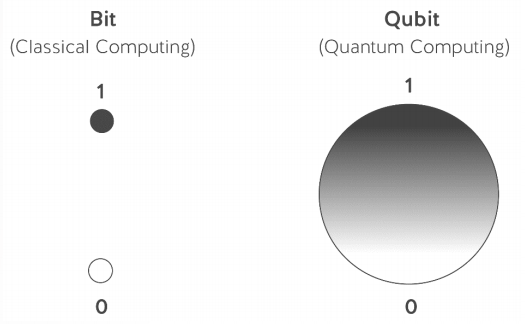
\includegraphics[width=0.8\textwidth]{figuras/bit_cubit.png}
	\caption{Estados de un bit y de cúbit \cite{clasica-vs-cuantica}}
	\label{fig:bit-cubit}
\end{figure}

El espacio de estados de un cúbit se puede representar mediante un espacio vectorial complejo bidimensional, al no ser práctico, se aprovecha el homeomorfismo entre la superficie de una esfera y el plano complejo cerrado con un punto en el infinito, dando lugar a lo que se conoce como la esfera de Bloch.\\

Una esfera de Bloch es una representación geométrica del espacio de estados puros de un sistema cuántico de dos niveles. Además se representa en el espacio $\mathds{R}^3$ por la esfera de radio unidad como se observa en la figura \ref{fig:esfera-bloch}, donde cada punto de la esfera es un posible estado del cúbit.\\


\begin{figure}[H]
	\centering
	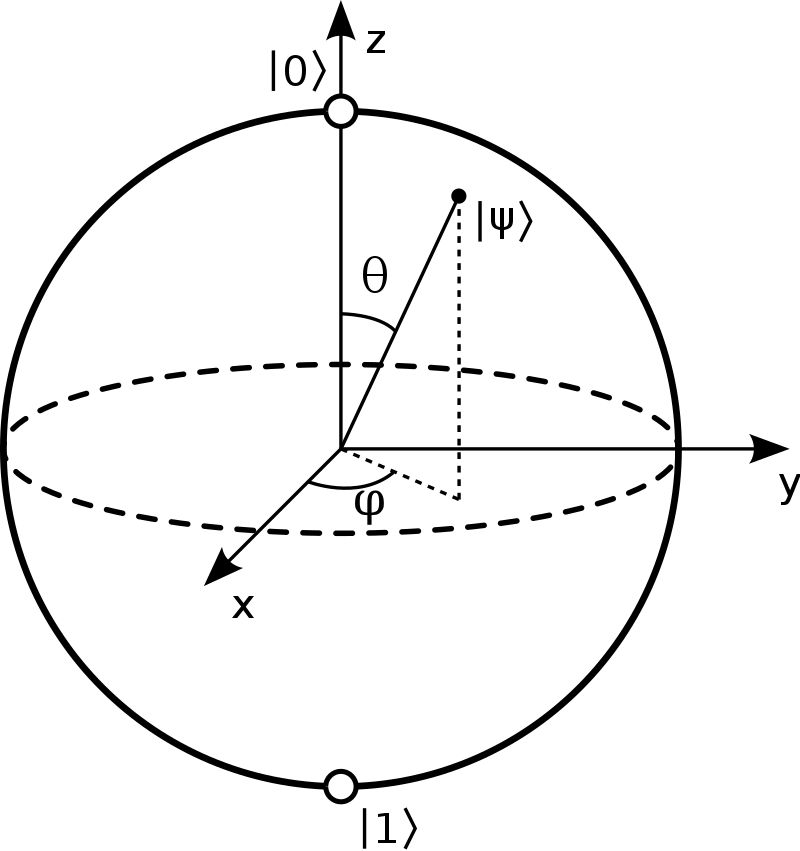
\includegraphics[width=0.4\textwidth]{figuras/esfera_bloch.png}
	\caption{Estructura cúbit, esfera de Bloch \cite{esfera-bloch}}
	\label{fig:esfera-bloch}
\end{figure}

\newpage
Un cúbit se puede representar como una combinación lineal de los estados $|0\rangle$ y $|1\rangle$, ecuación (\ref{eq:cubit}).\\

\begin{equation}\label{eq:cubit}
|\psi \rangle = \alpha|0\rangle + \beta |1\rangle
\end{equation}

Como $\alpha$ y $\beta$ son números complejos, la ecuación (\ref{eq:cubit}) se puede escribir en forma exponencial, ecuación (\ref{eq:cubit-expo}).\\

\begin{equation}\label{eq:cubit-expo}
|\psi\rangle = r_{\alpha} e^{i\phi_{\alpha}}|0\rangle + r_{\beta} e^{i\phi_{\beta}}|1\rangle\\
\end{equation}

\vspace{1em}
\subsection{Propiedades}
Entre las propiedades cuánticas destacan la superposición cuántica, el entrelazamiento cuántico y el teletransporte cuántico.\\

La \textbf{superposición cuántica} describe cómo una partícula puede estar en diferentes estados al mismo tiempo. Esto aporta gran capacidad de procesamiento, lo que hace posible resolver de manera eficiente problemas de mayor complejidad como la factorización de enteros, el algoritmo discreto y la simulación cuántica, que a día de hoy con los ordenadores clásicos son difíciles de romper.\\

Otro aspecto importante de la física cuántica relacionado con la superposición es el \textbf{entrelazamiento cuántico} de las partículas\cite{cumputacion-cuantica-clasica}. Esto es, si dos partículas en algún instante han interactuado retienen un tipo de conexión y pueden entrelazarse formando pares, de forma que al interactuar con una de las partículas, por muy separadas que estén, la otra se entera. Esto permite que aunque los cúbits estén separados interactúen entre sí. Con estos dos aspectos la capacidad de procesamiento aumenta considerablemente, cuántos más cúbits la capacidad de procesamiento aumenta considerablemente.\\

Por último, el \textbf{teletransporte cuántico} utiliza el entrelazamiento para enviar información de un lugar del espacio a otro sin necesidad de viajar a través de él.\\




\section{Blockchain}\label{sec:intro:blockchain}


\textit{Blockchain} es un sistemas de almacenamiento de información que se divide en bloques de datos enlazados mediante hash. A cada bloque se le asocia un hash a partir del bloque anterior, creando una lista enlazada, la búsqueda de información no es muy óptima si hay un número elevado de bloques. Para la búsqueda eficiente en \textit{blockchain} se usan los árboles de Merkle.\\

Los datos que almacena cada bloque son transacciones válidas, información referente a ese bloque y la relación con el bloque anterior mediante el \textit{hash}, por tanto el bloque tiene un lugar específico dentro de la cadena. De esta forma si hay una alteración en un determinado bloque se verá reflejado en su \textit{hash} y en el de los bloques posteriores, haciendo que la información de la cadena no se pueda perder, modificar o eliminar.\\


Los árboles de Merkle \cite{arbol-merkle} son una estructura de datos en árbol en el que cada nodo que no es hoja está etiquetado con el \textit{hash} que surge de la combinación de los valores o etiquetas de sus nodos hijo. Esta estructura permite que aunque los datos estén separados puedan ser ligados a un único valor de \textit{hash}, el \textit{hash} del nodo raíz del árbol. El \textit{hash} de este nodo va firmado para asegurar la integridad y hacer que la verificación sea fiable.\\

De esta forma se asegura que los datos son recibidos sin daños y sin ser alterados, además permite que los datos puedan ser entregados por partes, ya que un nodo puede obtener solo la cabecera de un bloque desde una fuente y otra pequeña parte del árbol desde otra fuente, pudiendo asegurar que los datos son correctos. Esto funciona porque si un usuario intenta hacer un cambio en una transacción falsa en la parte inferior del árbol en seguida se verá reflejado en la parte superior del árbol, es decir, en el nodo raíz. Esta propiedad se ve clara en la estructura del árbol de Merkle \ref{fig:arbol-Merkle}, donde los \textit{hash} de los nodos superiores se calculan a partir de los \textit{hash} de los nodos hijos.\\

\begin{figure}[H]
	\centering
	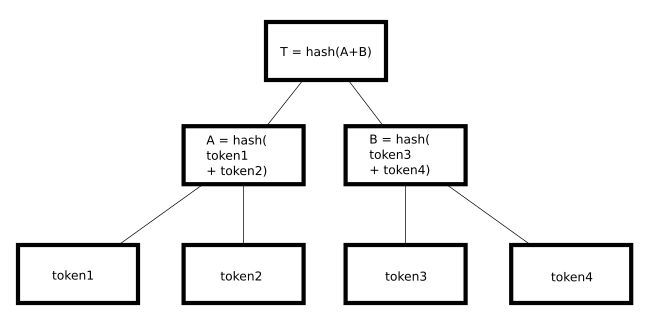
\includegraphics[width=0.8\textwidth]{figuras/arbol_merkle.png}
	\caption{Estructura de un árbol de Merkle \cite{img-arbol-merkle}}
	\label{fig:arbol-Merkle}
\end{figure}

La idea de la tecnología \textit{blockchain} surge a comienzos de 1991 cuando los científicos Stuart Haber y W. Scott Stornetta introducen una solución computacional para la firma de documentos digitales y que no pudieran ser modificados con el tiempo. Usaron cadenas de bloque para almacenar los documentos con sello de tiempo y en 1992 se incorporaron los árboles de Merkle, que podían recopilar varios documentos en un bloque haciendo el diseño más eficiente. Sin embargo, esta tecnología no se utilizó y la patente caducó en 2004 \cite{historia1-block}.\\

En 1998, Nick Szabo trabaja en una moneda digital descentralizada, ``bit gold''. Dos años después Stefan Konst publica su teoría sobre la seguridad criptográfica en las cadenas de bloques junto con algunas ideas de implementación \cite{historia2-block}.\\

En 2004, el informático y criptógrafo Harold Thomas Finney introdujo el sistema \acrshort{rpow} (prueba de trabajo reutilizable). El sistema se basa en \textit{HashCash} pero los token de prueba no están ligados a una aplicación sino que pueden ser gastados libremente como una moneda. Los clientes pueden crear tokens e intercambiarlos sin necesidad de regenerarlos \cite{RPoW}. \acrshort{rpow} resolvió el problema del doble gasto registrando los tokens en un servidor fiable diseñado para permitir a los usuarios verificar su exactitud e integridad en tiempo real. Este sistema puede considerarse como un prototipo de las criptomonedas.\\

A finales de 2008, un grupo de desarrolladores bajo el nombre de Satoshi Nakamoto publican un documento técnico en que se establece un modelo para \textit{blockchain}. Está basado en el algoritmo \acrshort{rpow} pero en lugar de usar dicho hardware, se utiliza un protocolo descentralizado peer-to-peer para verificar y rastrear las transacciones. En otras palabras los ``mineros'' extraen bitcoins para obtener una recompensa mediantes pruebas de trabajo y posteriormente los nodos los verifican. Bitcoin nació el 3 de enero de 2009 cuando Satoshi Nakamoto extrajo el primer bloque de bitcoin con una recompensa de 50 bitcoins. Y el 12 de enero de 2009 tuvo lugar la primera transacción entre Satoshi Nakamoto y Hal Finney que obtuvo 10 bitcoins.\\


A partir de 2014, se comienzan a explorar el potencial de las cadenas de bloque y a buscar otras aplicaciones fuera de su uso en las transacciones financieras.\\

Ethereum introduce programas informáticos que se ejecutan en la \textit{blockchain}, se pueden utilizar para realizar una transacción cumpliendo ciertas condiciones como los contratos inteligentes.\\

Los contratos inteligentes se tratan de contratos que tienen la capacidad de cumplirse de forma automática. Un contrato inteligente está constituido por un protocolo de códigos que permiten a un dispositivo ejecutar de forma automatizada las sentencias previamente programadas, prescindiendo de la intervención humana \cite{contrato-inteligente}.\\

\newpage
Además de los contratos inteligentes, Ethereum tiene su propia criptomoneda llamada Ether, se puede transferir entre cuentas y se utiliza para pagar las tarifas por la ejecución de los contratos inteligentes.\\

Otro proyecto de \textit{blockchain} a destacar es Hyperledger\cite{hyperledger-org}, iniciado en diciembre de $2015$ por la Fundación Linux. Hyperledger es una plataforma de código abierto centrada en el desarrollo de un conjunto de \textit{frameworks}, herramientas y bibliotecas para implementaciones de cadenas de bloques a nivel empresarial.\\

Hyperledger contiene varios \textit{frameworks} de contabilidad distribuidos, en los que se incluye Hyperledger Fabric, Sawtooth, Indy, así como herramientas como Hyperledger Caliper. Y bibliotecas como Hyperledger Ursa.\\

El proyecto Hyperledger pretende la mejora de aspectos como el rendimiento y fiabilidad de las empresas, además de agilizar los procesos comerciales de las industrias. Para ello ha de contar con el apoyo de las diferentes empresas (como Accenture, Fujitsu, IBM o Intel) formando así un proyecto colaborativo\cite{hyperledger-colab}.\\

Dentro de Hyperledger, el proyecto más destacado es Hyperledger Fabric. Este es uno de los dos proyectos originales de Hyperledger en el que colaboraba Digital Asset Holding, Blockstream e IBM. Es una \textit{blockchain} privada, de las más conocidas, que aspira a facilitar la implementación de cualquier modelo de uso. Además permite el despliegue de contratos inteligentes desarrollados en el lenguaje de programación de Google, ``Golang''. Dicha \textit{blockchain} posee un diseño muy flexible ya que permite crear contratos inteligentes en cualquier lenguaje o decidir qué algoritmo de consenso utilizar en la red (por defecto usa Practical Byzantine Fault Tolerance, \acrshort{pbft})\cite{hyperledger-fabric}.\\

Las cadenas de bloques o \textit{blockchain} permiten verificar, validar, rastrear todo tipo de información, ya sean contratos inteligentes, transacciones financieras, certificados digitales o firmas \cite{blockchain}, siendo estas últimas el centro de este trabajo. También permiten impulsar modificaciones orientadas a crear soluciones más robustas, por ejemplo en centros de salud o notarías que se explicarán más adelante.\\


Las \textit{blockchain} son vulnerables a futuros ataques cuánticos ya que su única línea de defensa es el algoritmo de firma de los bloques. Aunque, actualmente las cadenas de bloques son seguras, puesto que un ordenador clásico no tiene la capacidad de cómputo necesaria para descifrar cada bloque, obtener la información y volver a firmar todos los bloques sin dejar huella. Por eso para hacer una \textit{blockchain} resistente es necesario tener un criptosistema que no se pueda romper con computación cuántica, como por ejemplo el algoritmo \acrshort{uov}, ver apartado \ref{sec:intro:UOV}. \\

Los tres pilares de la tecnología \textit{blockchain} son la descentralización, transparencia e inmutabilidad \cite{pilares-blockchain}.\\

Un sistema centralizado almacena todos los datos en una misma entidad y habría que interactuar con la misma para obtener la información necesaria. Un ejemplo de un sistema centralizado son los bancos que almacenan todo el dinero y la única forma de pagar a alguien es a través de un banco. Es similar a la arquitectura cliente-servidor donde los clientes se comunican entre ellos mediante el servidor. Pero tener un único sitio para almacenar todos los datos es vulnerable a los ataques, informáticos, por otra parte si el nodo central se corrompe o tiene una actualización, los datos será incorrectos o no se podrán acceder a ellos. De los contras de los sistemas centralizados surge la idea de los sistemas \textbf{descentralizados}, la información no la tiene un único nodo sino que todos los usuarios son dueños de la información. La principal ideología de las \textit{blockchain} es poder interactuar usuario con usuario sin tener que pasar por un tercero.\\

El concepto \textbf{transparencia} se refiere a la transparencia de los datos no de las identidades. Esto es la identidad de la persona se oculta a través de la criptografía y lo único que se ve es su dirección pública, pero podemos ver todas las transacciones que se han realizado en su dirección pública. En el historial de transacciones no vemos ``Antonio envió 1BTC'' sino que aparece ``\sloppy{1MF1bhsFLkBzzz9vpFYEmvwT2TbyCt7NZJ} envió un 1BTC''. Este nivel de transparencia nunca antes había existido en el sistema financiero, lo que exige más responsabilidad a las grandes empresas. De la misma forma podemos trasladar este concepto fuera del sistema financiero por ejemplo a las cadenas de suministro, y saber exactamente de donde provienen los alimentos de un restaurante.\\

La \textbf{inmutabilidad} en el contexto de las cadenas de bloques significa que una vez introducida una transacción en la \textit{blockchain} ya no se puede alterar. De esta forma aplicando esta tecnología a los bancos se evitarían casos de malversación de fondos. Esta propiedad se obtiene gracias a la función criptográfica \textit{hash}.\\

La función \textit{hash} es el resultado de aplicar una función que transforma un mensaje de longitud variable en uno de longitud fija. Esto es calcular el resto módulo $n$ con $n$ la longitud fija. Al aplicar la función hash a un fichero, si se modifica algún dato del mismo cambiará su hash y por tanto se sabrá si ha sido manipulado desde que se envió, consiguiendo la integridad del mensaje.\\

De la misma forma si hay un cambio en una de las transacciones de un bloque se reflejará en el \textit{hash} del bloque, afectado a todos los bloques anteriores. Así si el atacante quiere preservar la integridad deberá de modificar todos los bloques siendo una tarea imposible. De esta forma se obtiene la inmutabilidad de los datos.\\

Hoy en día, la tecnología \textit{blockchain} está ganando mucha atención, no limitándose solo al uso en las criptomonedas. Así las cadenas de bloques tienen diversas aplicaciones entre ellas se encuentra la salud o la firma de documentos en las notarías. En el primer caso, cada centro  de salud podría tener el historial médico de cualquier paciente, de una forma segura y evitando falsificaciones, estos historiales se encontrarían en nodos distribuidos de forma descentralizada así se obtendría un acceso rápido y seguro. El segundo caso será en el que nos centraremos a lo largo de este proyecto. Hoy día la firma de documentos o transacciones por parte de un usuario es un problema puesto que se pueden copiar con facilidad, pero con \textit{blockchain} no podrían ser falsificadas debido a la propiedad de validación y rastreo de los datos.\\

\subsection{Blockchain ARK}

ARK es un ecosistema de criptomonedas descentralizado diseñado para aumentar la adopción de la tecnología \textit{blockchain} por parte de los usuarios. Se busca que la implementación de la cadena de bloques sea eficiente y fácil, y de esta forma poder usar dicha plataforma como puente inteligente entre varias cadenas de bloques no necesariamente de ARK. Cualquier desarrollador puede programar ARK, puesto que admite varios lenguajes de programación como \texttt{Python}, \texttt{Elixer}, \texttt{Java} o \texttt{API TypeScript} entre otros. El \textit{core} de la \textit{blockchain} que se ha utilizado se encuentra en \texttt{TypeScript}.\\

Algunas ventajas de la \textit{blockchain} ARK son, tener una interfaz de usuario intuitiva para extender el uso a la vida cotidiana, crear puentes inteligentes para posibilitar la comunicación entre diferentes \textit{blockchain}, admitir varios lenguajes de programación, facilidad para duplicar la cadena de bloques para permitir que se utilice para necesidades personales y por último, los coste de red son bastante bajos\cite{ark-pros}.\\

Hay dos motivos principales por los que se ha elegido esta \textit{blockchain} ARK y no otra. En primer lugar, la cadena de bloques es completamente de código abierto, permite a cualquier persona poder contribuir. Y en segundo lugar, su arquitectura modular permitiendo personalizar la aplicación para alcanzar nuestro objetivo (modificar el algoritmo de firma y verificación).\\


Un logro significativo del ecosistema ARK es brindar soporte a los contratos inteligentes directamente desde la cadena de bloques ARK utilizando puentes inteligentes. La capacidad de crear, lanzar y administrar contratos inteligentes entre dos tecnologías \textit{blockchain} diferentes sin ningún problema, abre el campo de posibilidades para crear soluciones comerciales.\\

Hyperledger Fabric agrega soporte al núcleo ARK v2 para contratos inteligentes. Dicho núcleo de ARK con toda la integración se ejecuta en los nodos conectados a la cadena de bloques principal de ARK. También la cadena Hyperledger personalizada puede agregarse a los mismos nodos o a un conjunto de nodos independientes\cite{hyperledger-ark}.\\



\section{Algoritmo UOV}\label{sec:intro:UOV}

El algoritmo aceite y vinagre desequilibrado\cite{algoritmo-UOV} es una versión simplificada del algoritmo aceite y vinagre, ambos algoritmos de firma digital. Para crear las firmas y validarlas es necesario resolver un sistema con $m$ ecuaciones y $n$ variables, que es un problema NP-duro\cite{UOV-def}, lo que significa que si fuésemos capaces de resolverlo con un ordenador cuántico, todos los problemas considerados en la actualidad serían vulnerables. Si $m$ y $n$ son casi iguales o iguales será más difícil resolver el sistema, obteniendo de esta forma un algoritmo de firma resistente a ataques cuánticos.\\

La principal ventaja del algoritmo \acrshort{uov} es que es un algoritmo post-cuántico, a diferencia de otros esquemas de firmas como \acrshort{rsa}, \acrshort{dsa}, basado en el logaritmo discreto, y su variante para curvas elípticas \mbox{\acrshort{ecdsa}} que no permanecerían seguros ante un ordenador cuántico. Esto se debe a que en la actualidad no existe un algoritmo eficiente para la resolución de sistemas multivariados de ecuaciones  en ordenador cuántico. Otra ventaja es la simplicidad de las operaciones utilizadas, ya que las firmas se crean y validan con operaciones de suma y multiplicaciones de valores pequeños, lo que requiere bajos recursos \textit{hardware}. 

Aunque el algoritmo usa sistemas pequeños y la longitud de las firmas son pequeñas, se necesitan claves públicas bastante más grandes en comparación con otros algoritmos de firma como \mbox{\acrshort{ecdsa}}, pudiendo ocupar dicha clave pública varios kilobytes de almacenamiento. Por otro lado ya se conocen algunos métodos de ataque, probablemente aparecerán más si se empieza a comercializar.\\

\subsection{Cuerpos finitos}
Se trabajará con el cuerpo finito de 128 elementos, $\mathds{F}_{2^7}$, extensión de grado $7$ del cuerpo $\mathds{F}_2$ de los enteros módulo $2$
 
\begin{equation}
\mathds{F}_{128} = \frac{\mathds{F}_2[x]}{\langle x^7 + x + 1 \rangle}
\end{equation}

Además el orden del cuerpo de las unidades es $127$, que es primo. Entonces todo elemento del cuerpo distinto de $1$ es un elemento primitivo, es decir, un generador.\\

La tabla \ref{tab:rel} muestra una representación de los elementos no nulos del cuerpo. En la implementación se ha utilizado la representación como cadena de bits, puesto que a la hora de trabajar es más fácil con una cadena de bits que con los polinomios.

\begin{table}[h]
	\begin{center}
		\begin{tabular}{p{0.2\linewidth}p {0.2\linewidth}p{0.2\linewidth}}
			\textbf{Polinomio} & \textbf{Bits} & \textbf{$\log_a$}\\
			\toprule
				$1$ & [0, 0, 0, 0, 0, 0, 1] & 0\\
				$a$ & [0, 0, 0, 0, 0, 1, 0] & 1\\
				$a^2$ & [0, 0, 0, 0, 1, 0, 0] & 2\\
				\\
				$\vdots$ & $\vdots$ & $\vdots$\\
				\\
				$a^6 + a^5 + a^4 + 1$ & [1, 1, 1, 0, 0, 0, 1] & 124\\
				$a^6 + a^5 + 1$ & [1, 1, 0, 0, 0, 0, 1] & 125\\
				$a^6 + 1$ & [1, 0, 0, 0, 0, 0, 1] & 126\\
			\bottomrule
		\end{tabular}
	\end{center}
	\caption{Representación de los elementos no nulos de $\mathds{F}_{128}$}
	\label{tab:rel}
\end{table}

La implementación del cuerpo finito de $2^7$ elementos no se ha realizado de forma genérica sino para que sea específica para el algoritmo \acrshort{uov}, de esta forma es mucho más sencillo implementar la aritmética del cuerpo. Para la suma en $\mathds{F}_2$ sólo tenemos que fijarnos que es lo mismo que el operador lógico \textit{XOR}, mientras que para el producto, al encontrarnos en un cuerpo como un orden pequeño, se usarán unas tablas que contienen las correspondencias entre los elementos no nulos del cuerpo y sus logaritmos en base $a$, por lo que el producto se convierte en una suma módulo $127$.\\




\subsection{Parámetros y fórmula}
Para empezar se indican los parámetros que serán de utilidad para entender el algoritmo.
\begin{itemize}
	\item r: Grado del cuerpo extendido, $\mathds{F}_2 \subset \mathds{F}_{2^r}$. En la implementación se va tomar $r$ igual a $7$, pero se puede realizar con cualquier valor de $r$ sin un esfuerzo adicional.
	\item $m$: Tamaño de la clave pública, además del número de variables de aceite.
	\item $v$: Número de variables vinagre.
	\item $n$: Número total de variables, las de aceite más las de vinagre.
	\item $x$: Vector de $n$ componentes, denominando a las primeras $v$ componentes  $x_1, \dotsb, x_v$ vinagre y al resto aceites.
	
	
	%\item $\mathcal{H}$: Función salida extensible se usa para crear el hash del mensaje y proviene de la clave pública.
	%\item $\mathcal{G}$: Función salida extensible se usa para la generación de la clave pública a partir de una semilla privada.
\end{itemize}

El esquema de la firma UOV utiliza la función unidireccional $\mathcal{P}: \mathds{F}_{2^r}^n \rightarrow \mathds{F}_{2^r}^m$, que es una función cuadrática multivariante en $n = m + v$ variables. Esta función se puede descomponer como $\mathcal{P} = \mathcal{F} \circ \mathcal{T}$, donde $\mathcal{T}: \mathds{F}_{2^r}^n \rightarrow \mathds{F}_{2^r}^n$ es linear invertible, y $\mathcal{F}: \mathds{F}_{2^r}^n \rightarrow \mathds{F}_{2^r}^m$  función cuadrática cuyas $m$ componentes son de la forma:

\begin{equation}\label{eq:fun}
f_k(x) = \sum_{i=1}^v \sum_{j=i}^n \alpha_{i,j,k} x_i x_j + \sum_{i=1}^n \beta_{i,k} x_i
\end{equation}
donde $\alpha_{i,j,k}$ y $\beta_{i,k}$ se toman aleatoriamente en $\mathds{F}_2$ siendo $\left(\alpha_{i,j,k}\right)_{\begin{subarray}{l}{1\leqslant i \leqslant v }\\ {1 \leqslant j \leqslant n}\end{subarray}}$ un vector de matrices triangulares superiores. De esta manera será más eficiente y no afectará a la seguridad del algoritmo. Se entiende por matriz triangular superior, una matriz no necesariamente cuadrada que tiene debajo de la primera diagonal valores nulos. Las primeras $v$ variables, $x_1,\cdots,x_v$ son las variables vinagres y las $m$ variables restantes son las variables aceite.



\subsection{Generación de la clave privada}
La clave privada viene dada para cada una de las $m$ ecuaciones, es decir, para cada $k$ se tiene una matriz de dimensiones $v \times n$, $\left(\alpha_{i,j,k}\right)_{\begin{subarray}{l}{1\leqslant i \leqslant v }\\ {1 \leqslant j \leqslant n}\end{subarray}}$, y un vector de $v$ componentes, $\left(\beta_{i,k}\right)_{1\leqslant i \leqslant v }$, cuyos valores son elegidos de forma aleatoria en $\mathds{F}_2$.


\subsection{Generación de la clave pública}
La clave pública se va a definir para cada $k\in \{1, \dots, m\}$ de la siguiente manera, 

\begin{itemize}
	\item ${\alpha_{pub}}_k = \left(
	\begin{array}{c}
	I_v \\
	\hline
	T'_{v \times m}
	\end{array}
	\right) \left(\alpha_{i,j,k}\right)_{\begin{subarray}{l}{1 \leqslant i\leqslant v }\\ {i\leqslant j \leqslant n}\end{subarray}} \ T$
	
	\item ${\beta_{pub}}_k = \left(\beta_{j,k}\right)_{1\leqslant j\leqslant n}\ T$
\end{itemize}

Ahora se va a justificar porqué se toman estos valores de la clave pública. Primero se pasan las $m$ ecuaciones (\ref{eq:fun}) a forma matricial, ecuación (\ref{eq:matriz}). La notación a seguir para las matrices transpuestas es $X^{\scriptscriptstyle T}$, con $X$ una matriz.

\begin{equation}\label{eq:matriz} 
	f_k(x) = x^v\ \left(\alpha_{i,j,k}\right)_{\begin{subarray}{l}{1\leqslant i \leqslant v }\\ {i \leqslant j \leqslant n}\end{subarray}}\ \left(x^v, x^m \right)^{\scriptscriptstyle T} + \left(\beta_{i,k}\right)_{1\leqslant i \leqslant v }\ \left(x^v, x^m\right)^{\scriptscriptstyle T}
\end{equation}
siendo $x^v$ los vinagres y $x^m$ los aceites, por tanto $x$ se puede expresar como $\big(x^v, x^m\big)^{\scriptscriptstyle T}$.\\


Para generar la clave pública es necesario incluir una nueva matriz $T$ con la forma que muestra la ecuación (\ref{mat:T}), a esta matriz se le denomina matriz de distorsión. La matriz de distorsión se incluye para aumentar la seguridad del algoritmo y así sea más complejo calcular la función inversa $\mathcal{P}$.

\begin{equation}
	T =
	\Bigg(
	\begin{array}{c|c}
	I_v & T_{v\times m} \\
	\hline
	0 & I_m
	\end{array}
	\Bigg)
	\label{mat:T}
\end{equation}

Además la matriz de distorsión cumple la igualdad $T\cdot s^{\scriptscriptstyle T} = x ^{\scriptscriptstyle T}$, donde $s$ es la firma del mensaje, y despejando $x$ se obtiene la ecuación (\ref{eq:def-x}).

\begin{equation}
	x =  s \cdot T^{\scriptscriptstyle T} = s  \left(
	\begin{array}{c|c}
	I_v & 0 \\
	\hline
	T^{\scriptscriptstyle T}_{v \times m} & I_m
	\end{array}
	\right)
	= \left(s^v, s^m\right) \left(
	\begin{array}{c|c}
	I_v & 0 \\
	\hline
	T^{\scriptscriptstyle T}_{v \times m} & I_m
	\end{array}
	\right)
	= \left(s^v + s^m T^{\scriptscriptstyle T}_{v\times m}, s^m \right)
	\label{eq:def-x}
\end{equation}

Sustituyendo la anterior definición de $x$ en la ecuación (\ref{eq:matriz}), se llega a la ecuación (\ref{eq:sus-def-x}).

\begin{equation}
	f_k(x) = s  
	\left(\begin{array}{c}
		I_v \\
		\hline
		T^{\scriptscriptstyle T}_{v \times m}
	\end{array}\right)
	\left(\alpha_{i,j,k}\right)_{\begin{subarray}{l}{1\leqslant i \leqslant v }\\ {i \leqslant j \leqslant n}\end{subarray}}\ T \ s^{\scriptscriptstyle T} + 
	\left(\beta_{j,k}\right)_{1\leqslant j\leqslant n}\ T\ s^{\scriptscriptstyle T}
	\label{eq:sus-def-x}
\end{equation}
donde $k \in \{1,\dots,m\}$


\subsection{Algoritmo de firma}

Para calcular la firma es necesario conocer los valores de la clave privada $\alpha$ y $\beta$, tomar de forma aleatoria los del vinagre $x^v$, puesto que estos son fijos y no variables pasarán a denominarse como $a^v$, y coger los $m$ primeros bits del \textit{hash} del mensaje $h_k$.

Para facilitar los cálculos se multiplican los vinagres por $\alpha$ y se obtiene \mbox{$A_k = a^v\ \left(\alpha_{i,j,k}\right)_{\begin{subarray}{l}{1 \leqslant i\leqslant v }\\ {1\leqslant j \leqslant n}\end{subarray}} = \left(A^v_k, A^m_k\right)$}. Si se sustituye este resultado en la ecuación (\ref{eq:matriz}) y se despejan los aceites, se llega a la ecuación (\ref{eq:despeje}). Este despeje se puede realizar sin problema, debido a que el sistema de ecuaciones se vuelve lineal cuando las variables de vinagre son fijas y ninguna variable de aceite se multiplica por otra de aceite. Por tanto se puede resolver usando, por ejemplo, el algoritmo de reducción gaussiano.

\begin{align}
h_k &= A_k^v\ (a^v)^{\scriptscriptstyle T} +  A_k^m\ (x^m)^{\scriptscriptstyle T} + \beta_k^v\ (a^v)^{\scriptscriptstyle T} + \beta_k^m\ (x^m)^{\scriptscriptstyle T}\\
\label{eq:ter-coef}
(A_k^m + \beta_k^m) (x^m)^{\scriptscriptstyle T} &= h_k - (A_k^v + \beta_k^v) (a^v)^{\scriptscriptstyle T}\\
\label{eq:despeje}
(x^m)^{\scriptscriptstyle T} &= (A_k^m + \beta_k^m)^{-1} (h_k - (A_k^v + \beta_k^v) (a^v)^{\scriptscriptstyle T})
\end{align}
Si $(A_k^m + \beta_k^m)$ fuese una matriz singular, entonces se tomarían otros valores de vinagres.

De esta forma se han calculado los aceites, esto es, las últimas $m$ componentes del vector $x$. Para calcular la firma, $s$, se hace uso de la definición de $x$  dada en la ecuación (\ref{eq:def-x}), puesto que solo es necesario realizar un simple despeje. Por otro lado, se tiene que  que $T$ es igual a su inversa, gracias a la definición de $T$ y teniendo en cuenta que la matriz toma valores en $\mathds{F}_2$.

\begin{equation}\label{eq:firma}
	s = x \cdot {T^{\scriptscriptstyle T}}^{-1} = x \cdot T ^{\scriptscriptstyle T}
\end{equation}
donde $x = \big(x^v, x^m\big)$ con $x^v$ son los vinagres aleatorios y $x^m$ los aceites.




\subsection{Algoritmo de verificación}

Para comprobar que el mensaje es correcto y que no ha sufrido ninguna transformación durante el envío del mismo, se utiliza una versión del sistema utilizado para la firma. Se hace modificación para que el atacante no pueda obtener la clave privada ni las variables de aceite y vinagre. Para cada $k \in  \{1,\dots, m\}$ se tiene que cumplir la igualdad (\ref{eq:veri}).


\begin{equation}\label{eq:veri}
	h_k = \ {\alpha_{pub}}_k \ s^{\scriptscriptstyle T} + {\beta_{pub}}_{k} \ s^{\scriptscriptstyle T}
\end{equation}

\subsection{Ejemplo}

Se muestra un ejemplo para mejor comprensión del algoritmo \acrshort{uov} utilizando valores de $m$ y $v$ pequeños, ambos con valor $3$, y dejando fijo el valor de $r$ igual a $7$.

Generamos la clave privada con valores aleatorios. Notamos que las matrices del vector $\alpha_{priv}$, ecuación (\ref{eq:ej-alpha-priv}), son matrices triangulares superiores de dimensión $3\ \times\ 6$, esto es dimensión $m\ \times\ n$. Además el número de matrices es $3$ el valor de $v$.

\begin{equation}\label{eq:ej-alpha-priv}
{\alpha_{priv}} = 
	\Bigg(\begin{matrix}
	\Big(\begin{smallmatrix}
		1 & 0 & 1 & 1 & 1 & 0\\
		0 & 0 & 0 & 0 & 1 & 1\\
		0 & 0 & 0 & 1 & 1 & 1
	\end{smallmatrix}\Big)
		
	\Big(\begin{smallmatrix}
		1 & 1 & 0 & 1 & 1 & 0\\
		0 & 0 & 1 & 1 & 1 & 0\\
		0 & 0 & 1 & 1 & 1 & 1
	\end{smallmatrix}\Big)
	
	\Big(\begin{smallmatrix}
		0 & 0 & 0 & 1 & 0 & 0\\
		0 & 0 & 1 & 1 & 0 & 1\\
		0 & 0 & 0 & 0 & 1 & 1
	\end{smallmatrix}\Big)
	\end{matrix}\Bigg)
\end{equation}

La segunda parte de la clave privada es $\beta_{priv}$, consta de un vector de $3$ vectores, donde cada uno tiene $n$ componentes, esto es $6$ componentes, ecuación (\ref{eq:ej-beta-priv}).

\begin{equation}\label{eq:ej-beta-priv}
{\beta_{priv}} = 
	\left(\begin{matrix}
		\left(\begin{smallmatrix}
			1 & 0 & 0 & 1 & 0 & 0
		\end{smallmatrix}\right)
	
		\left(\begin{smallmatrix}
			0 & 0 & 1 & 0 & 1 & 0
		\end{smallmatrix}\right)
	
		\left(\begin{smallmatrix}
			1 & 1 & 0 & 1 & 0 & 1
		\end{smallmatrix}\right)
	\end{matrix}\right)
\end{equation}


La forma de la matriz T viene dada por la ecuación \ref{mat:T}, la del ejemplo se muestra en la ecuación (\ref{eq:ej-T})

\begin{equation}\label{eq:ej-T}
{T} =
	\left(\begin{array}{c|c}
	\\
	\ \ \ \ \ I_3\ \ \ \ & \ \ \ \ T_{3\times 3} \ \ \  \\
	\\
	\hline
	\\
	0 & I_3\\
	\\
	\end{array}\right) =
	\left(\begin{array}{c|c}
		1\ \ 0\ \ 0\ & 0\ \ 0\ \ 0\\
		0\ \ 1\ \ 0\ & 0\ \ 0\ \ 1\\
		0\ \ 0\ \ 1\ & 1\ \ 0\ \ 1\\
		\hline
		0\ \ 0\ \ 0\ & 1\ \ 0\ \ 0\\
		0\ \ 0\ \ 0\ & 0\ \ 1\ \ 0\\
		0\ \ 0\ \ 0\ & 0\ \ 0\ \ 1
	\end{array}\right)
\end{equation}


Clave pública consta de dos partes $\alpha_{pub}$ y $\beta_{pub}$. Cada  componente de $\alpha_{pub}$ se calculan multiplicando tres matrices, una matriz, que tiene dos partes la $I_3$ y $T'_{3\times 3}$, por la $k-ésima$ componente de $\alpha_{priv}$ y por $T$.

\begin{equation}\label{eq:ej-alpha-pub-1}
	\begin{aligned}
	{{\alpha_{pub}}_1}  & =  
	\left(\begin{matrix}
		1 & 0 & 0\\
		0 & 1 & 0\\
		0 & 0 & 1\\
		\hline
		0 & 0 & 1\\
		0 & 0 & 0\\
		0 & 1 & 1
	\end{matrix}\right)
	\cdot
	\begin{pmatrix}
		1 & 0 & 1 & 1 & 1 & 0\\
		0 & 0 & 0 & 0 & 1 & 1\\
		0 & 0 & 0 & 1 & 1 & 1
	\end{pmatrix}
	\cdot
	\left(\begin{array}{c|c}
		1\ \ 0\ \ 0\ & 0\ \ 0\ \ 0\\
		0\ \ 1\ \ 0\ & 0\ \ 0\ \ 1\\
		0\ \ 0\ \ 1\ & 1\ \ 0\ \ 1\\
		\hline
		0\ \ 0\ \ 0\ & 1\ \ 0\ \ 0\\
		0\ \ 0\ \ 0\ & 0\ \ 1\ \ 0\\
		0\ \ 0\ \ 0\ & 0\ \ 0\ \ 1
	\end{array}\right) \\
	& = \left(\begin{array}{c|c}
		1\ \ 0\ \ 1\ & 1\ \ 1\ \ 0\\
		0\ \ 0\ \ 0\ & 0\ \ 1\ \ 1\\
		0\ \ 0\ \ 0\ & 1\ \ 1\ \ 1\\
		\hline
		0\ \ 0\ \ 0\ & 1\ \ 1\ \ 1\\
		0\ \ 0\ \ 0\ & 0\ \ 0\ \ 0\\
		0\ \ 0\ \ 0\ & 1\ \ 0\ \ 0\\
	\end{array}\right)
	\cdot
	\left(\begin{array}{c|c}
		1\ \ 0\ \ 0\ & 0\ \ 0\ \ 0\\
		0\ \ 1\ \ 0\ & 0\ \ 0\ \ 1\\
		0\ \ 0\ \ 1\ & 1\ \ 0\ \ 1\\
		\hline
		0\ \ 0\ \ 0\ & 1\ \ 0\ \ 0\\
		0\ \ 0\ \ 0\ & 0\ \ 1\ \ 0\\
		0\ \ 0\ \ 0\ & 0\ \ 0\ \ 1
	\end{array}\right)\\
	& = \begin{pmatrix}
		1 & 0 & 1 & 0 & 1 & 1\\
		0 & 0 & 0 & 0 & 1 & 1\\
		0 & 0 & 0 & 1 & 1 & 1\\
		0 & 0 & 0 & 1 & 1 & 1\\
		0 & 0 & 0 & 0 & 0 & 0\\
		0 & 0 & 0 & 1 & 0 & 0
	\end{pmatrix}
	\end{aligned}
\end{equation}

De la misma forma se obtiene ${\alpha_{pub}}_2$ y ${\alpha_{pub}}_3$, así la ecuación (\ref{eq:ej-alpha-pub}) muestra el resultado de $\alpha_{pub}$.


\begin{equation}\label{eq:ej-alpha-pub}
{\alpha_{pub}} = 
	\left(\begin{matrix}
	\left(\begin{smallmatrix}
		1 & 0 & 1 & 0 & 1 & 1\\
		0 & 0 & 0 & 0 & 1 & 1\\
		0 & 0 & 0 & 1 & 1 & 1\\
		0 & 0 & 0 & 1 & 1 & 1\\
		0 & 0 & 0 & 0 & 0 & 0\\
		0 & 0 & 0 & 1 & 0 & 0
	\end{smallmatrix}\right)
		
	\left(\begin{smallmatrix}
		1 & 1 & 0 & 1 & 1 & 1\\
		0 & 0 & 1 & 0 & 1 & 1\\
		0 & 0 & 1 & 0 & 1 & 0\\
		0 & 0 & 1 & 0 & 1 & 0\\
		0 & 0 & 0 & 0 & 0 & 0\\
		0 & 0 & 0 & 0 & 0 & 1
	\end{smallmatrix}\right)
	
	\left(\begin{smallmatrix}
		0 & 0 & 0 & 1 & 0 & 0\\
		0 & 0 & 1 & 0 & 0 & 0\\
		0 & 0 & 0 & 0 & 1 & 1\\
		0 & 0 & 0 & 0 & 1 & 1\\
		0 & 0 & 0 & 0 & 0 & 0\\
		0 & 0 & 1 & 0 & 1 & 1
	\end{smallmatrix}\right)
	\end{matrix}\right)
\end{equation}


Ahora se calcula $\beta_{pub}$ para ello se va a realizar el cálculo de la primera componente del vector ${\beta_{pub}}_1$ a modo de ejemplo, multiplicando la primera componente de $\beta_{priv}$ por $T$, ecuación (\ref{eq:ej-beta-pub-1}).

\begin{equation}\label{eq:ej-beta-pub-1}
	{{\beta_{pub}}_1} = 
	\left(\begin{matrix}1 & 0 & 0 & 1 & 0 & 0\end{matrix}\right) \cdot
	\left(\begin{array}{c|c}
		1\ \ 0\ \ 0\ & 0\ \ 0\ \ 0\\
		0\ \ 1\ \ 0\ & 0\ \ 0\ \ 1\\
		0\ \ 0\ \ 1\ & 1\ \ 0\ \ 1\\
		\hline
		0\ \ 0\ \ 0\ & 1\ \ 0\ \ 0\\
		0\ \ 0\ \ 0\ & 0\ \ 1\ \ 0\\
		0\ \ 0\ \ 0\ & 0\ \ 0\ \ 1
	\end{array}\right) =
	\left(\begin{matrix}1 & 0 & 0 & 1 & 0 & 0\end{matrix}\right)
\end{equation}

De manera análoga se calculan el resto de componentes, ${\beta_{pub}}_2$ y ${\beta_{pub}}_3$, para obtener el vector completo $\beta_{pub}$, ecuación (\ref{eq:ej-beta-pub}).

\begin{equation}\label{eq:ej-beta-pub}
{\beta_{pub}} = 
	\left(\begin{matrix}
		\left(\begin{smallmatrix}
			1 & 0 & 0 & 1 & 0 & 0
		\end{smallmatrix}\right)
	
		\left(\begin{smallmatrix}
			0 & 0 & 1 & 1 & 1 & 1
		\end{smallmatrix}\right)
	
		\left(\begin{smallmatrix}
			1 & 1 & 0 & 1 & 0 & 0
		\end{smallmatrix}\right)
	\end{matrix}\right)
\end{equation}

Llegados a este punto comienza el proceso de firma del mensaje, en este caso el mensaje al que se le va a realizar la firma es \texttt{"{}Este mensaje es un mensaje de prueba. Quiero se sea un poco largo para que se aprecie el efecto de la función hash"{}}, el hash de dicho mensaje calculado con la función \texttt{sha256} es \texttt{"{}c2f"{}}, la ecuación (\ref{eq:ej-hash}) contiene el \textit{hash} en $\mathds{F}_{128}$.

\begin{equation}\label{eq:ej-hash}
	{hash} = 
	\left(\begin{matrix}
		\left(\begin{smallmatrix}
			0 & 0 & 0 & 1 & 1 & 0 & 0
		\end{smallmatrix}\right)
		
		\left(\begin{smallmatrix}
			0 & 0 & 0 & 0 & 0 & 1 & 0
		\end{smallmatrix}\right)
		
		\left(\begin{smallmatrix}
			0 & 0 & 0 & 1 & 1 & 1 & 1
		\end{smallmatrix}\right)
	\end{matrix}\right)
\end{equation}

Los vinagres se han tomado de forma aleatoria, ecuación (\ref{eq:ej-vinegar}). 

\begin{equation}\label{eq:ej-vinegar}
{a^v} = 
	\left(\begin{matrix}
		\left(\begin{smallmatrix}
			0 & 1 & 1 & 0 & 1 & 0 & 0
		\end{smallmatrix}\right)
	
		\left(\begin{smallmatrix}
			1 & 1 & 1 & 1 & 1 & 0 & 0
		\end{smallmatrix}\right)
	
		\left(\begin{smallmatrix}
			1 & 1 & 1 & 1 & 0 & 0 & 1
		\end{smallmatrix}\right)
	\end{matrix}\right)
\end{equation}

La $k-ésima$ matriz del vector $A$ es el resultado de multiplicar el vinagre por la matriz ${\alpha_{priv}}_k$ donde $k$ se mueve entre $1$ y $3$, para lo cual, es necesario extender los componentes de las matrices de $\alpha_{priv}$, que se encuentran en $\mathds{F}_{2}$, al cuerpo $\mathds{F}_{128}$. En el ejemplo no se ha puesto la matriz extendida para entender mejor la multiplicación y no perderse con los vectores, finalmente la multiplicación será el vector nulo si se multiplica por $0$ o el mismo vector cuando se multiplique por $1$.

\begin{equation}\label{eq:ej-A-1}
	\begin{aligned}
	{A_1} & = 
		\left(\begin{matrix}
			\left(\begin{smallmatrix}
				0 & 1 & 1 & 0 & 1 & 0 & 0
			\end{smallmatrix}\right)
	
			\left(\begin{smallmatrix}
				1 & 1 & 1 & 1 & 1 & 0 & 0
			\end{smallmatrix}\right)
		
			\left(\begin{smallmatrix}
				1 & 1 & 1 & 1 & 0 & 0 & 1
			\end{smallmatrix}\right)
		\end{matrix}\right)
		\cdot
		\left(\begin{smallmatrix}
			1 & 0 & 1 & 1 & 1 & 0\\
			0 & 0 & 0 & 0 & 1 & 1\\
			0 & 0 & 0 & 1 & 1 & 1
		\end{smallmatrix}\right)\\
		& = \left(\begin{matrix}
				\left(\begin{smallmatrix}
					0 & 1 & 1 & 0 & 1 & 0 & 0
				\end{smallmatrix}\right)
		
				\left(\begin{smallmatrix}
					0 & 0 & 0 & 0 & 0 & 0 & 0
				\end{smallmatrix}\right)
		
				\left(\begin{smallmatrix}
					0 & 1 & 1 & 0 & 1 & 0 & 0
				\end{smallmatrix}\right)
			
				\left(\begin{smallmatrix}
					1 & 0 & 0 & 1 & 1 & 0 & 1
				\end{smallmatrix}\right)
				\left(\begin{smallmatrix}
					0 & 1 & 1 & 0 & 0 & 0 & 1
				\end{smallmatrix}\right)
				\left(\begin{smallmatrix}
					0 & 0 & 0 & 0 & 1 & 0 & 1
				\end{smallmatrix}\right)
			\end{matrix}\right)
	\end{aligned}
\end{equation}

Calculando el resto de las componentes se obtiene la matriz $A$, ecuación (\ref{eq:ej-A}).

\begin{equation}\label{eq:ej-A}
	\begin{aligned}
	{A} = & \bigg(\begin{matrix}\left(\begin{matrix}
				\left(\begin{smallmatrix}
					0 & 1 & 1 & 0 & 1 & 0 & 0
				\end{smallmatrix}\right)
		
				\left(\begin{smallmatrix}
					0 & 0 & 0 & 0 & 0 & 0 & 0
				\end{smallmatrix}\right)
		
				\left(\begin{smallmatrix}
					0 & 1 & 1 & 0 & 1 & 0 & 0
				\end{smallmatrix}\right)
			
				\left(\begin{smallmatrix}
					1 & 0 & 0 & 1 & 1 & 0 & 1
				\end{smallmatrix}\right)
				
				\left(\begin{smallmatrix}
					0 & 1 & 1 & 0 & 0 & 0 & 1
				\end{smallmatrix}\right)
				
				\left(\begin{smallmatrix}
					0 & 0 & 0 & 0 & 1 & 0 & 1
				\end{smallmatrix}\right)
			\end{matrix}\right)\end{matrix}\bigg.\\
			&
			\bigg.\begin{matrix}\left(\begin{matrix}
				\left(\begin{smallmatrix}
					0 & 1 & 1 & 0 & 1 & 0 & 0
				\end{smallmatrix}\right)
		
				\left(\begin{smallmatrix}
					0 & 1 & 1 & 0 & 1 & 0 & 0
				\end{smallmatrix}\right)
		
				\left(\begin{smallmatrix}
					0 & 0 & 0 & 0 & 1 & 0 & 1
				\end{smallmatrix}\right)
				
				\left(\begin{smallmatrix}
					0 & 1 & 1 & 0 & 0 & 0 & 1
				\end{smallmatrix}\right)
				
				\left(\begin{smallmatrix}
					0 & 1 & 1 & 0 & 0 & 0 & 1
				\end{smallmatrix}\right)
				
				\left(\begin{smallmatrix}
					1 & 1 & 1 & 1 & 0 & 0 & 1
				\end{smallmatrix}\right)
			\end{matrix}\right)\end{matrix}\bigg.\\
			& \bigg.\begin{matrix}\left(\begin{matrix}
				\left(\begin{smallmatrix}
					0 & 0 & 0 & 0 & 0 & 0 & 0
				\end{smallmatrix}\right)
		
				\left(\begin{smallmatrix}
					0 & 0 & 0 & 0 & 0 & 0 & 0
				\end{smallmatrix}\right)
		
				\left(\begin{smallmatrix}
					1 & 1 & 1 & 1 & 1 & 0 & 0
				\end{smallmatrix}\right)
				
				\left(\begin{smallmatrix}
					1 & 0 & 0 & 1 & 0 & 0 & 0
				\end{smallmatrix}\right)
				
				\left(\begin{smallmatrix}
					1 & 1 & 1 & 1 & 0 & 0 & 1
				\end{smallmatrix}\right)
				
				\left(\begin{smallmatrix}
					0 & 0 & 0 & 0 & 1 & 0 & 1
				\end{smallmatrix}\right)
			\end{matrix}\right)\end{matrix}\bigg)\\
	\end{aligned}	
\end{equation}

Los coeficientes se obtienen de la suma de las últimas $m$ componentes, en este caso las $3$ últimas, de cada $A_k$ con ${\beta_{priv}}_k$. Pero tenemos el mismo problema de antes, puesto que los coeficientes de $A_k$ pertenecen a $\mathds{F}_{128}$ y los coeficientes de ${\beta_{priv}}_k$ se encuentra en $\mathds{F}_2$, por tanto lo que vamos a sumar es $0$ o $1$, o lo que es lo mismo realizar la operación lógica $XOR$ con los elementos $\left(\begin{smallmatrix}0 & 0 & 0 & 0 & 0 & 0 & 0\end{smallmatrix}\right)$ o $\left(\begin{smallmatrix}0 & 0 & 0 & 0 & 0 & 0 & 1\end{smallmatrix}\right)$, ecuación (\ref{eq:ej-coef}).

\begin{equation}\label{eq:ej-coef}
	{coef} =
	\left(\begin{matrix}
		\left(\begin{matrix}
			\left(\begin{smallmatrix}1 & 0 & 0 & 1 & 1 & 0 & 0\end{smallmatrix}\right)\\
			\left(\begin{smallmatrix}0 & 1 & 1 & 0 & 0 & 0 & 1\end{smallmatrix}\right)\\
			\left(\begin{smallmatrix}0 & 0 & 0 & 0 & 1 & 0 & 1\end{smallmatrix}\right)
		\end{matrix}\right)
		\left(\begin{matrix}
			\left(\begin{smallmatrix}0 & 1 & 1 & 0 & 0 & 0 & 1\end{smallmatrix}\right)\\
			\left(\begin{smallmatrix}0 & 1 & 1 & 0 & 0 & 0 & 0\end{smallmatrix}\right)\\
			\left(\begin{smallmatrix}1 & 1 & 1 & 1 & 0 & 0 & 1\end{smallmatrix}\right)
		\end{matrix}\right)
		\left(\begin{matrix}
			\left(\begin{smallmatrix}1 & 0 & 0 & 1 & 0 & 0 & 1\end{smallmatrix}\right)\\
			\left(\begin{smallmatrix}1 & 1 & 1 & 1 & 0 & 0 & 1\end{smallmatrix}\right)\\
			\left(\begin{smallmatrix}0 & 0 & 0 & 0 & 1 & 0 & 0\end{smallmatrix}\right)
		\end{matrix}\right)
	\end{matrix}\right)
\end{equation}

Los términos corresponden a la parte de la derecha de la ecuación (\ref{eq:ter-coef}), a continuación se va a realizar el cálculo para $k$ igual $1$. La ecuación (\ref{eq:ej-beta-1-v}) corresponde al primer vector de $\beta$, $\left(\begin{array}{c}1\ 0\ 0\ 1\ 0\ 0\end{array}\right)$, donde se han transformado los elementos de $\mathds{F}_2$ a $\mathds{F}_{128}$ y se han tomado las $3$ primeras componentes.

\begin{equation}\label{eq:ej-beta-1-v}
	{\beta^v_1} = 
		\left(\begin{matrix}
			\left(\begin{smallmatrix}0 & 0 & 0 & 0 & 0 & 0 & 1\end{smallmatrix}\right)			
			\left(\begin{smallmatrix}0 & 0 & 0 & 0 & 0 & 0 & 0\end{smallmatrix}\right)
			\left(\begin{smallmatrix}0 & 0 & 0 & 0 & 0 & 0 & 0\end{smallmatrix}\right)
		\end{matrix}\right)
\end{equation}

De la misma forma se han tomado las $3$ primeras componentes del primer vector de $A$, ecuación (\ref{eq:ej-A-1-v}).

\begin{equation}\label{eq:ej-A-1-v}
	{A^v_1} = 
		\left(\begin{matrix}
			\left(\begin{smallmatrix}0 & 1 & 1 & 0 & 1 & 0 & 0\end{smallmatrix}\right)			
			\left(\begin{smallmatrix}0 & 0 & 0 & 0 & 0 & 0 & 0\end{smallmatrix}\right)
			\left(\begin{smallmatrix}0 & 1 & 1 & 0 & 1 & 0 & 0\end{smallmatrix}\right)
		\end{matrix}\right)
\end{equation}

El vector $sum$ contiene la suma de $A^v_1$ y $\beta^v_1$, ecuación (\ref{eq:ej-sum}).

\begin{equation}\label{eq:ej-sum}
	{sum} = 
		\left(\begin{matrix}
			\left(\begin{smallmatrix}0 & 1 & 1 & 0 & 1 & 0 & 1\end{smallmatrix}\right)			
			\left(\begin{smallmatrix}0 & 0 & 0 & 0 & 0 & 0 & 0\end{smallmatrix}\right)
			\left(\begin{smallmatrix}0 & 1 & 1 & 0 & 1 & 0 & 0\end{smallmatrix}\right)
		\end{matrix}\right)
\end{equation}

Finalmente, para calcular $term$ hay que multiplicar $sum$ por $a^v$ y restárselo a la primera componente de $hash$. Al realizar las operaciones módulo $2$, la resta y la suma son lo mismo, por tanto se realizará la operación lógica \textit{XOR} con el $hash$, ecuación (\ref{eq:ej-ter-1}).

\begin{equation}\label{eq:ej-ter-1}
	\begin{split}
	{term_1} &= 
		\left(\begin{matrix}
			\left(\begin{smallmatrix}0 & 1 & 1 & 0 & 1 & 0 & 1\end{smallmatrix}\right)			
			\left(\begin{smallmatrix}0 & 0 & 0 & 0 & 0 & 0 & 0\end{smallmatrix}\right)
			\left(\begin{smallmatrix}0 & 1 & 1 & 0 & 1 & 0 & 0\end{smallmatrix}\right)
		\end{matrix}\right) \cdot 
		\left(\begin{matrix}
			\left(\begin{smallmatrix}0 & 1 & 1 & 0 & 1 & 0 & 0\end{smallmatrix}\right)\\
			\left(\begin{smallmatrix}1 & 1 & 1 & 1 & 1 & 0 & 0\end{smallmatrix}\right)\\
			\left(\begin{smallmatrix}1 & 1 & 1 & 1 & 0 & 0 & 1\end{smallmatrix}\right)\\
		\end{matrix}\right)
		+ \left(\begin{smallmatrix}1 & 0 & 1 & 1 & 0 & 0 & 0\end{smallmatrix}\right)\\
		&= \left(\begin{smallmatrix}0 & 0 & 0 & 1 & 1 & 0 & 0\end{smallmatrix}\right) + 
		\left(\begin{smallmatrix}1 & 0 & 1 & 1 & 0 & 0 & 0\end{smallmatrix}\right)\\
		& = \left(\begin{smallmatrix}1 & 0 & 1 & 0 & 1 & 0 & 0\end{smallmatrix}\right)
	\end{split}
\end{equation}

De la misma forma se calculan el resto de los términos llegando al vector $term$, ecuación (\ref{eq:ej-ter}).

\begin{equation}\label{eq:ej-ter}
	{term} = 
		\left(\begin{matrix}
			\left(\begin{smallmatrix}1 & 0 & 1 & 0 & 1 & 0 & 0\end{smallmatrix}\right)			
			\left(\begin{smallmatrix}1 & 1 & 0 & 1 & 0 & 0 & 0\end{smallmatrix}\right)
			\left(\begin{smallmatrix}1 & 1 & 0 & 0 & 0 & 0 & 0\end{smallmatrix}\right)
		\end{matrix}\right)
\end{equation}

Tras la resolución del sistema $coef \cdot oil = term$ se han obtenido los aceites, ecuación (\ref{eq:ej-oil}).

\begin{equation}\label{eq:ej-oil}
	{oil} = 
		\left(\begin{matrix}
			\left(\begin{smallmatrix}0 & 0 & 0 & 0 & 1 & 1 & 0\end{smallmatrix}\right)			
			\left(\begin{smallmatrix}0 & 0 & 1 & 1 & 0 & 1 & 1\end{smallmatrix}\right)
			\left(\begin{smallmatrix}0 & 1 & 0 & 0 & 1 & 1 & 0\end{smallmatrix}\right)
		\end{matrix}\right)
\end{equation}

Ahora se forma el vector $aux$ uniendo los vinagres con los aceites, ecuación (\ref{eq:ej-aux}).

\begin{equation}\label{eq:ej-aux}
	\begin{aligned}
	{aux} = & 
		\left(\begin{matrix}
			\left(\begin{smallmatrix}0 & 0 & 0 & 0 & 1 & 1 & 0\end{smallmatrix}\right)		
			\left(\begin{smallmatrix}0 & 0 & 1 & 1 & 0 & 1 & 1\end{smallmatrix}\right)
			\left(\begin{smallmatrix}0 & 1 & 0 & 0 & 1 & 1 & 0\end{smallmatrix}\right)\end{matrix}\right.\\
			&\left.\begin{matrix}\left(\begin{smallmatrix}0 & 1 & 1 & 0 & 1 & 0 & 0\end{smallmatrix}\right)
			\left(\begin{smallmatrix}1 & 1 & 1 & 1 & 1 & 0 & 0\end{smallmatrix}\right)
			\left(\begin{smallmatrix}1 & 1 & 1 & 1 & 0 & 0 & 1\end{smallmatrix}\right)
		\end{matrix}\right)
	\end{aligned}
\end{equation}

La firma del mensaje se obtiene multiplicando el vector $aux$ por la inversa de $T$, que de la forma que está construida dicha matriz $T$ coincide con su inversa, ecuación (\ref{eq:ej-firma}).

\begin{equation}\label{eq:ej-firma}
	\begin{aligned}
	{firma} =&
		\left(\begin{matrix}
			\left(\begin{smallmatrix}0 & 1 & 1 & 0 & 1 & 0 & 0\end{smallmatrix}\right)			
			\left(\begin{smallmatrix}1 & 0 & 1 & 1 & 0 & 1 & 0\end{smallmatrix}\right)
			\left(\begin{smallmatrix}1 & 0 & 1 & 1 & 0 & 0 & 1\end{smallmatrix}\right)\end{matrix}\right.
			\\
			& \left.\begin{matrix}\left(\begin{smallmatrix}0 & 0 & 0 & 0 & 1 & 1 & 0\end{smallmatrix}\right)			
			\left(\begin{smallmatrix}0 & 0 & 1 & 1 & 0 & 1 & 1\end{smallmatrix}\right)
			\left(\begin{smallmatrix}0 & 1 & 0 & 0 & 1 & 1 & 0\end{smallmatrix}\right)
		\end{matrix}\right)
	\end{aligned}
\end{equation}

Para realizar la confirmación del mensaje es necesario calcular dos variables auxiliares, $\alpha_{aux}$ y $\beta_{aux}$.

Para calcular ${\alpha_{aux}}_1$ hay que multiplicar los vectores $firma$, ${\alpha_{pub}}_1$y $firma$ transpuesta, ecuación (\ref{eq:ej-aux-alpha-1}).

\begin{equation}\label{eq:ej-aux-alpha-1}
	\begin{aligned}
	{{\alpha_{aux}}_1} & = 
		\begin{pmatrix}firma\end{pmatrix}
		\cdot \left(\begin{smallmatrix}
			1 & 0 & 1 & 0 & 1 & 1\\
			0 & 0 & 0 & 0 & 1 & 1\\
			0 & 0 & 0 & 1 & 1 & 1\\
			0 & 0 & 0 & 1 & 1 & 1\\
			0 & 0 & 0 & 0 & 0 & 0\\
			0 & 0 & 0 & 1 & 0 & 0
		\end{smallmatrix}\right)
		\cdot \big(\begin{matrix}firma\end{matrix}\big)^{\scriptscriptstyle T}\\
		& = \left(\begin{smallmatrix}0 & 1 & 1 & 1 & 1 & 1 & 0\end{smallmatrix}\right)
	\end{aligned}
\end{equation}

La segunda variable ${\beta_{aux}}_k$ es el producto de la $k-ésima$ componente del vector $\beta_{pub}$, donde sus componentes se encuentran en $\mathds{F}_2$ y habrá que transformarlos en componentes de $\mathds{F}_{128}$, por el vector $firma$ transpuesta, ecuación (\ref{eq:ej-aux-beta-1}).

\begin{equation}\label{eq:ej-aux-beta-1}
	\begin{aligned}
	{{\beta_{aux}}_1} & = 
		\left(\begin{smallmatrix}1 & 0 & 0 & 1 & 0 & 0\end{smallmatrix}\right)
		\cdot \big(\begin{matrix}firma\end{matrix}\big)^{\scriptscriptstyle T}\\
		& = \left(\begin{smallmatrix}0 & 1 & 1 & 1 & 1 & 1 & 0\end{smallmatrix}\right)
	\end{aligned}
\end{equation}

Calculando todas la componentes de $\alpha_{aux}$ y $\beta_{aux}$ se obtienen los vectores las ecuaciones (\ref{eq:ej-aux-alpha}) y (\ref{eq:ej-aux-beta}), respectivamente.

\begin{equation}\label{eq:ej-aux-alpha}
	{\alpha_{aux}} = \left(\begin{matrix}
		\left(\begin{smallmatrix}0 & 1 & 1 & 1 & 1 & 1 & 0\end{smallmatrix}\right)
		\left(\begin{smallmatrix}1 & 1 & 0 & 0 & 0 & 0 & 0\end{smallmatrix}\right)
		\left(\begin{smallmatrix}1 & 1 & 0 & 0 & 1 & 1 & 1\end{smallmatrix}\right)
		\end{matrix}\right)
\end{equation}

\begin{equation}\label{eq:ej-aux-beta}
	{\beta_{aux}} =
		\left(\begin{matrix}
			\left(\begin{smallmatrix}0 & 1 & 1 & 0 & 0 & 1 & 0\end{smallmatrix}\right)		
			\left(\begin{smallmatrix}1 & 1 & 0 & 0 & 0 & 1 & 0\end{smallmatrix}\right)
			\left(\begin{smallmatrix}1 & 1 & 0 & 1 & 0 & 0 & 0\end{smallmatrix}\right)
		\end{matrix}\right)
\end{equation}

Sumando los vectores componente a componente, ecuación (\ref{eq:ej-suma}), anteriormente calculados, se obtiene vector a comparar con el $hash$ del mensaje. 

\begin{equation}\label{eq:ej-suma}
	\left(\begin{matrix}
		\left(\begin{smallmatrix}0 & 0 & 0 & 1 & 1 & 0 & 0\end{smallmatrix}\right)
		\left(\begin{smallmatrix}0 & 0 & 0 & 0 & 0 & 1 & 0\end{smallmatrix}\right)
		\left(\begin{smallmatrix}0 & 0 & 0 & 1 & 1 & 1 & 1\end{smallmatrix}\right)
	\end{matrix}\right)
\end{equation}

Si el mensaje no ha sido corrompido habrá de ser igual que el $hash$ del mensaje, ecuación (\ref{eq:ej-verif}).

\begin{equation}\label{eq:ej-verif}
	\begin{aligned}
	\left(\begin{matrix}
		\left(\begin{smallmatrix}0 & 0 & 0 & 1 & 1 & 0 & 0\end{smallmatrix}\right)
		\left(\begin{smallmatrix}0 & 0 & 0 & 0 & 0 & 1 & 0\end{smallmatrix}\right)
		\left(\begin{smallmatrix}0 & 0 & 0 & 1 & 1 & 1 & 1\end{smallmatrix}\right)
	\end{matrix}\right)==\left(\begin{matrix}
		\left(\begin{smallmatrix}0 & 0 & 0 & 1 & 1 & 0 & 0\end{smallmatrix}\right)
		\left(\begin{smallmatrix}0 & 0 & 0 & 0 & 0 & 1 & 0\end{smallmatrix}\right)
		\left(\begin{smallmatrix}0 & 0 & 0 & 1 & 1 & 1 & 1\end{smallmatrix}\right)
	\end{matrix}\right)
	\end{aligned}
\end{equation}




